\documentclass{article}
\usepackage{graphicx, tikz-cd, float, titlepic, booktabs} % Required for inserting images
\usepackage{pgfplots}
\pgfplotsset{compat=1.15}
\usepackage{mathrsfs}
\usetikzlibrary{arrows}
\usepackage{amsmath, amssymb, amsthm, amsfonts, siunitx, physics, gensymb}
\AtBeginDocument{\RenewCommandCopy\qty\SI}
\usepackage[version=4]{mhchem}
\usepackage[most,many,breakable]{tcolorbox}
\usepackage{fancyhdr, varwidth}
\usepackage[table,xcdraw]{xcolor}
\usepackage[Glenn]{fncychap}
%Options: Sonny, Lenny, Glenn, Conny, Rejne, Bjarne, Bjornstrup
\usepackage{hyperref, cleveref}
\usepackage{icomma, enumitem} %comma as decimal and continue enumerate with [resume]
\usepackage[danish]{babel}
%%%%%%%%%%%%%%%%%%%%%%%%%%%%%%
% SELF MADE COLORS
%%%%%%%%%%%%%%%%%%%%%%%%%%%%%%
\definecolor{myg}{RGB}{56, 140, 70}
\definecolor{myb}{RGB}{45, 111, 177}
\definecolor{myr}{RGB}{199, 68, 64}
\definecolor{mytheorembg}{HTML}{F2F2F9}
\definecolor{mytheoremfr}{HTML}{00007B}
\definecolor{mylenmabg}{HTML}{FFFAF8}
\definecolor{mylenmafr}{HTML}{983b0f}
\definecolor{mypropbg}{HTML}{f2fbfc}
\definecolor{mypropfr}{HTML}{191971}
\definecolor{myexamplebg}{HTML}{F2FBF8}
\definecolor{myexamplefr}{HTML}{88D6D1}
\definecolor{myexampleti}{HTML}{2A7F7F}
\definecolor{mydefinitbg}{HTML}{E5E5FF}
\definecolor{mydefinitfr}{HTML}{3F3FA3}
\definecolor{notesgreen}{RGB}{0,162,0}
\definecolor{myp}{RGB}{197, 92, 212}
\definecolor{mygr}{HTML}{2C3338}
\definecolor{myred}{RGB}{127,0,0}
\definecolor{myyellow}{RGB}{169,121,69}
\definecolor{myexercisebg}{HTML}{F2FBF8}
\definecolor{myexercisefg}{HTML}{88D6D1}
%%%%%%%%%%%%%%%%%%%%%%%%%%%%%%%%%%%%%%%%%%%%%%%%%%%%%%%%%%%%%%%%%%%%%%
% Box environments for theorems and problems
%%%%%%%%%%%%%%%%%%%%%%%%%%%%%%%%%%%%%%%%%%%%%%%%%%%%%%%%%%%%%%%%%%%%%
\setlength{\parindent}{1cm}
%================================
% Question BOX
%================================
\makeatletter
\newtcbtheorem{question}{Opgave}{enhanced,
	breakable,
	colback=white,
	colframe=myb!80!black,
	attach boxed title to top left={yshift*=-\tcboxedtitleheight},
	fonttitle=\bfseries,
	title={#2},
	boxed title size=title,
	boxed title style={%
			sharp corners,
			rounded corners=northwest,
			colback=tcbcolframe,
			boxrule=0pt,
		},
	underlay boxed title={%
			\path[fill=tcbcolframe] (title.south west)--(title.south east)
			to[out=0, in=180] ([xshift=5mm]title.east)--
			(title.center-|frame.east)
			[rounded corners=\kvtcb@arc] |-
			(frame.north) -| cycle;
		},
	#1
}{def}
\makeatother
%================================
% DEFINITION BOX
%================================

\newtcbtheorem[]{Definition}{Definition}{enhanced,
	before skip=2mm,after skip=2mm, colback=red!5,colframe=red!80!black,boxrule=0.5mm,
	attach boxed title to top left={xshift=1cm,yshift*=1mm-\tcboxedtitleheight}, varwidth boxed title*=-3cm,
	boxed title style={frame code={
					\path[fill=tcbcolback]
					([yshift=-1mm,xshift=-1mm]frame.north west)
					arc[start angle=0,end angle=180,radius=1mm]
					([yshift=-1mm,xshift=1mm]frame.north east)
					arc[start angle=180,end angle=0,radius=1mm];
					\path[left color=tcbcolback!60!black,right color=tcbcolback!60!black,
						middle color=tcbcolback!80!black]
					([xshift=-2mm]frame.north west) -- ([xshift=2mm]frame.north east)
					[rounded corners=1mm]-- ([xshift=1mm,yshift=-1mm]frame.north east)
					-- (frame.south east) -- (frame.south west)
					-- ([xshift=-1mm,yshift=-1mm]frame.north west)
					[sharp corners]-- cycle;
				},interior engine=empty,
		},
	fonttitle=\bfseries,
	title={#2},#1}{def}
\newtcbtheorem[]{definition}{Definition}{enhanced,
	before skip=2mm,after skip=2mm, colback=red!5,colframe=red!80!black,boxrule=0.5mm,
	attach boxed title to top left={xshift=1cm,yshift*=1mm-\tcboxedtitleheight}, varwidth boxed title*=-3cm,
	boxed title style={frame code={
					\path[fill=tcbcolback]
					([yshift=-1mm,xshift=-1mm]frame.north west)
					arc[start angle=0,end angle=180,radius=1mm]
					([yshift=-1mm,xshift=1mm]frame.north east)
					arc[start angle=180,end angle=0,radius=1mm];
					\path[left color=tcbcolback!60!black,right color=tcbcolback!60!black,
						middle color=tcbcolback!80!black]
					([xshift=-2mm]frame.north west) -- ([xshift=2mm]frame.north east)
					[rounded corners=1mm]-- ([xshift=1mm,yshift=-1mm]frame.north east)
					-- (frame.south east) -- (frame.south west)
					-- ([xshift=-1mm,yshift=-1mm]frame.north west)
					[sharp corners]-- cycle;
				},interior engine=empty,
		},
	fonttitle=\bfseries,
	title={#2},#1}{def}

\newtcbtheorem{theo}%
    {Theorem}{}{theorem}
\newtcolorbox{prob}[1]{colback=red!5!white,colframe=red!50!black,fonttitle=\bfseries,title={#1}}
%================================
% NOTE BOX
%================================

\usetikzlibrary{arrows,calc,shadows.blur}
\tcbuselibrary{skins}
\newtcolorbox{note}[1][]{%
	enhanced jigsaw,
	colback=gray!20!white,%
	colframe=gray!80!black,
	size=small,
	boxrule=1pt,
	title=\textbf{Note:},
	halign title=flush center,
	coltitle=black,
	breakable,
	drop shadow=black!50!white,
	attach boxed title to top left={xshift=1cm,yshift=-\tcboxedtitleheight/2,yshifttext=-\tcboxedtitleheight/2},
	minipage boxed title=1.5cm,
	boxed title style={%
			colback=white,
			size=fbox,
			boxrule=1pt,
			boxsep=2pt,
			underlay={%
					\coordinate (dotA) at ($(interior.west) + (-0.5pt,0)$);
					\coordinate (dotB) at ($(interior.east) + (0.5pt,0)$);
					\begin{scope}
						\clip (interior.north west) rectangle ([xshift=3ex]interior.east);
						\filldraw [white, blur shadow={shadow opacity=60, shadow yshift=-.75ex}, rounded corners=2pt] (interior.north west) rectangle (interior.south east);
					\end{scope}
					\begin{scope}[gray!80!black]
						\fill (dotA) circle (2pt);
						\fill (dotB) circle (2pt);
					\end{scope}
				},
		},
	#1,
}

%%%%%%%%%%%%%%%%%%%%%%%%%%%%%%%%%%%%%%%%%%%%%%%%%%%%%%%%%%%%%%%%%
% SELF MADE COMMANDS
%%%%%%%%%%%%%%%%%%%%%%%%%%%%%%
\newcommand{\sol}{\setlength{\parindent}{0cm}\textbf{\textit{Løsning:}}\setlength{\parindent}{1cm}}
%%%%%%%%%%%%%%%%%%%%%%%%%%%%%%%%%
\usepackage[tmargin=2cm,rmargin=1in,lmargin=1in,margin=0.85in,bmargin=2cm,footskip=.2in]{geometry}\pagestyle{fancy}
\lhead{Minrui Kevin Zhou 2.b}
\rhead{Aflevering 27}

\title{Aflevering 27\\
{\Large \textbf{2.b mat A}}}
\author{Kevin Zhou}
\date{\today}

\begin{document}
\maketitle
\section*{Bedømmelseskriterier:}
\begin{itemize}
    \setlength\itemsep{3cm}
    \Large
    \item  Redegørelse og dokumentation for metode
    \item Figurer, grafer og andre illustrationer
    \item Notation og layout
    \item Formidling og forklaring
\end{itemize}
\pagebreak
\begin{question}{Opgave 6}{}
  En funktion $f:]-3;2] \to \mathbb{R}$ er givet ved
  \[
  f(x)= 2x^3+3x^2-12x+6
  \] 
  \begin{itemize}
    \item[a.] Bestem ekstrema for $f$
  \end{itemize}
\end{question}
\sol \\
\textbf{a.}
Vi finder først den afledede funktion for $f$ med hensyn til $x$.
\[
f'(x)=6x^2+6x-12
\] 
Vi finder nu løsningen til ligningen $f'(x)=0$.
\begin{equation*}
\begin{split}
  f'(x)=0 &\iff 6x^2+6x-12=0 \\
  &\implies x=\frac{-6-\sqrt{6^2-4 \cdot 6 \cdot (-12)} }{2 \cdot 6} \lor x=\frac{-6+\sqrt{6^2-4 \cdot 6 \cdot (-12)} }{2 \cdot 6}\\ 
  &\iff x=\frac{-6-18}{2 \cdot 6} \lor x=\frac{-6+18}{2 \cdot 6}\\ 
  &\iff x=-2 \lor x=1
\end{split}
\end{equation*}
Vi finder nu den dobbeltafledede funktion for $f$ og tager den af de to løsninger til $f'(x)=0$.
\begin{equation*}
\begin{split}
  f''(x)=12x+6 
\end{split}
\end{equation*}
Vi har altså
\begin{equation*}
\begin{split}
  f''(-2)&=-18<0\\ 
  f''(1)&=18>0
\end{split}
\end{equation*}
-2 må da være et maksimumssted og 1 må være et minimumssted.
Vi kan da beregne ekstrema for $f$ ved at tage $f$ af de to fundne ekstremumssteder. 
\begin{equation*}
\begin{split}
  &f(-2)=26\\ 
  &f(1)=-1
\end{split}
\end{equation*}
Altså er ekstrema for $f$ 26 og -1. 
\begin{question}{Opgave 7}{}
  Lad funktionen $f$ være givet ved
  \[
  f(x)=x-x^3
  \] 
  \begin{itemize}
    \item[a.] Bestem en ligning for tangenten til grafen for $f$ i punktet $\left(-1,f(-1)\right)$.
  \end{itemize}
  Den tangent, hvis ligning blev bestemt i \textbf{a.} kaldes t.
  \begin{itemize}
    \item[b.] Angiv koordinatsættet til hvert af de to punkter, hvor tangenten $t$ skærer grafen for $f$. 
  \end{itemize}
\end{question}
\sol \\
\textbf{a.}
Ligningen for tangenten til grafen for $f$ i punktet $\left(-1,f(-1)\right)$ må da være
\begin{equation*}
\begin{split}
  y&=f'(-1)\cdot (x-(-1))+f(-1)\\ 
  &=\left(1-3 \cdot (-1)^2\right) \cdot (x+1)+0\\ 
  &=-2x-2
\end{split}
\end{equation*}
Altså er ligningen for denne tangent $y=-2x-2$.\\[1ex]
\textbf{b.}
Ved skæring for tangenten med grafen for $f$ må der gælde følgende, hvor vi løser ligningen med nulreglen
\begin{equation*}
\begin{split}
  x-x^3=-2x-2 &\iff -x^3+3x+2=0\\ 
  &\iff (x-2)\cdot (x^2+2x+1)=0\\ 
  &\iff (x-2) \cdot (x+1)^2=0\\
  &\iff x=2 \lor x=-1
\end{split}
\end{equation*}
Vi finder nu de to tilhørende y-værdier til punkterne.
\begin{equation*}
\begin{split}
  x=2 &\implies y=-2 \cdot 2 -2=-6\\ 
  x=-1 &\implies y=-2 \cdot (-1)-2=0
\end{split}
\end{equation*}
Koordinatsættet til de to punkter, hvor $t$ skærer grafen for $f$ må da være $(2,-6)$ og $(-1,0)$.
\begin{question}{Opgave 8}{}
  Tabellen i \cref{tab:tab} viser nogle sammenhørende værdier af alderen og højden for en bestemt abe.
  I en model antages sammenhængen mellem en abes alder og højde at være givet ved 
  \[
  f(x)= ax^2+bx+c, \quad 0 \leq x \leq 7
  \] 
  hvor $x$ er abens alder målt i år og $f(x)$ er abens højde målt i \unit{cm}.
  \begin{itemize}
    \item[a.] Bestem tallene $a, b \text{ og } c$ via tallene i tabellen. 
    \item[b.] Benyt modellen til at bestemme abens højde, når den er 7 år gammel.
    \item[c.] Bestem $f'(4)$ og giv en fortolkning af dette tal.
  \end{itemize}
\end{question}
\begin{table}[H]
\centering
\begin{tabular}{@{}llllllll@{}}
\toprule
Alder/år & 0  & 1  & 2  & 3  & 4  & 5  & 6  \\ \midrule
Højde/cm & 30 & 37 & 43 & 47 & 51 & 54 & 56 \\ \bottomrule
\end{tabular}
\caption{Værdier for alderen og højden for en bestemt abe}
\label{tab:tab}
\end{table}
\sol \\
\textbf{a.}
Vi laver da en regressionsanalyse med LoggerPro, der bruger mindste kvadraters metode.
Denne ses i \cref{fig:abe}.
\begin{figure}[H]
\begin{center}
  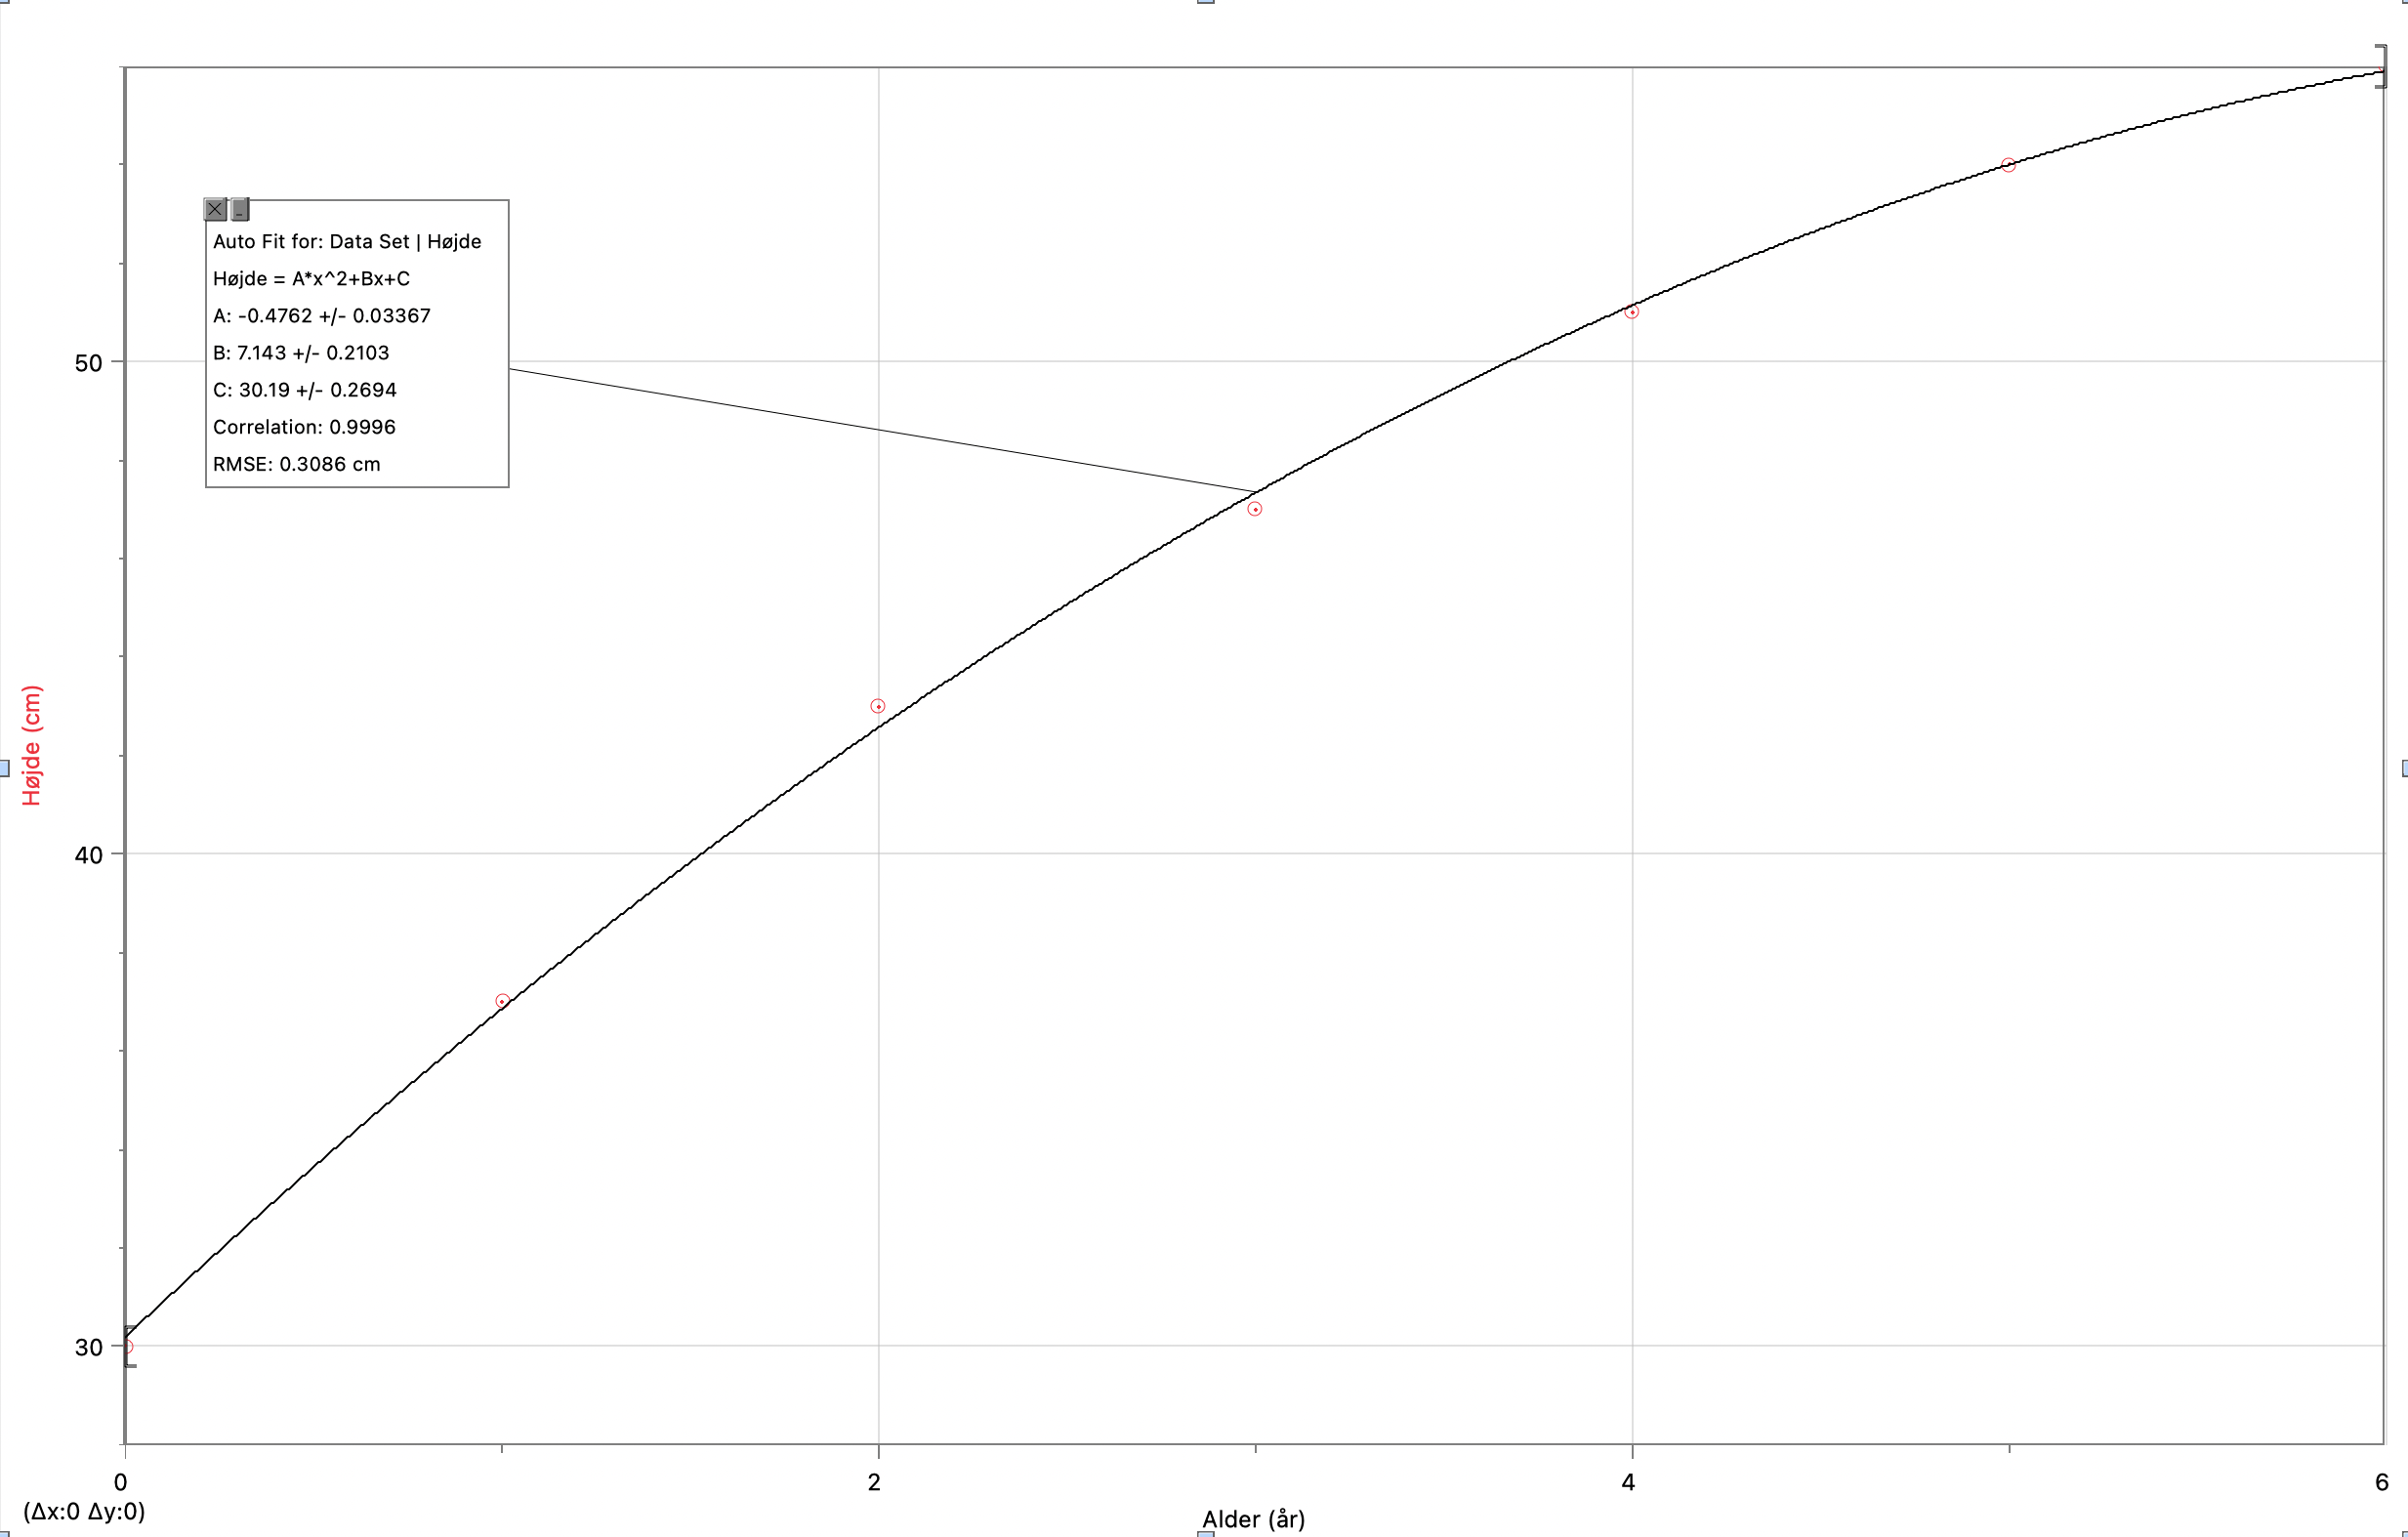
\includegraphics[width=\textwidth]{abe.png}
\end{center}
\caption{Regressionsanalyse lavet i LoggerPro}
\label{fig:abe}
\end{figure}
Vi ser da, at vi får 
\begin{equation*}
\begin{split}
  a&=-0,4762 \\
  b&=7,143 \\ 
  c&= 30,19
\end{split}
\end{equation*}
\textbf{b.}
For at bestemme abens højde, når den er 7 år gammel, tager vi funktionen $f$ af $7$. 
\begin{equation*}
\begin{split}
  f(7)&=-0,4762 \cdot 7^2 + 6,143 \cdot 7 + 30,19\\ 
  &\approx 50
\end{split}
\end{equation*}
Altså er højden på en 7-årig abe $50 \;\unit{cm} $.\\[1ex]
\textbf{c.}
Vi bestemmer først den afledede funktion for $f$.
\begin{equation*}
\begin{split}
  f'(x)&=\dv{x} \left(-0,4762 \cdot x^2 + 6,143 \cdot x + 30,19\right) \\ 
  &=-0,9524 \cdot x + 6,143
\end{split}
\end{equation*}
Vi tager nu den afledede funktion for $f$ af 4. 
\begin{equation*}
\begin{split}
  f'(4)&=-0,9524 \cdot 4+6,143\\
  &=2,3334
\end{split}
\end{equation*}
Dette tal fortæller, at aben vokser med $2,3334$ cm per år, når aben er fire år. 
\end{document}
